% Options for packages loaded elsewhere
\PassOptionsToPackage{unicode}{hyperref}
\PassOptionsToPackage{hyphens}{url}
\PassOptionsToPackage{dvipsnames,svgnames,x11names}{xcolor}
%
\documentclass[
  letterpaper,
  DIV=11,
  numbers=noendperiod]{scrartcl}

\usepackage{amsmath,amssymb}
\usepackage{iftex}
\ifPDFTeX
  \usepackage[T1]{fontenc}
  \usepackage[utf8]{inputenc}
  \usepackage{textcomp} % provide euro and other symbols
\else % if luatex or xetex
  \usepackage{unicode-math}
  \defaultfontfeatures{Scale=MatchLowercase}
  \defaultfontfeatures[\rmfamily]{Ligatures=TeX,Scale=1}
\fi
\usepackage{lmodern}
\ifPDFTeX\else  
    % xetex/luatex font selection
\fi
% Use upquote if available, for straight quotes in verbatim environments
\IfFileExists{upquote.sty}{\usepackage{upquote}}{}
\IfFileExists{microtype.sty}{% use microtype if available
  \usepackage[]{microtype}
  \UseMicrotypeSet[protrusion]{basicmath} % disable protrusion for tt fonts
}{}
\makeatletter
\@ifundefined{KOMAClassName}{% if non-KOMA class
  \IfFileExists{parskip.sty}{%
    \usepackage{parskip}
  }{% else
    \setlength{\parindent}{0pt}
    \setlength{\parskip}{6pt plus 2pt minus 1pt}}
}{% if KOMA class
  \KOMAoptions{parskip=half}}
\makeatother
\usepackage{xcolor}
\usepackage[margin=2cm]{geometry}
\setlength{\emergencystretch}{3em} % prevent overfull lines
\setcounter{secnumdepth}{5}
% Make \paragraph and \subparagraph free-standing
\makeatletter
\ifx\paragraph\undefined\else
  \let\oldparagraph\paragraph
  \renewcommand{\paragraph}{
    \@ifstar
      \xxxParagraphStar
      \xxxParagraphNoStar
  }
  \newcommand{\xxxParagraphStar}[1]{\oldparagraph*{#1}\mbox{}}
  \newcommand{\xxxParagraphNoStar}[1]{\oldparagraph{#1}\mbox{}}
\fi
\ifx\subparagraph\undefined\else
  \let\oldsubparagraph\subparagraph
  \renewcommand{\subparagraph}{
    \@ifstar
      \xxxSubParagraphStar
      \xxxSubParagraphNoStar
  }
  \newcommand{\xxxSubParagraphStar}[1]{\oldsubparagraph*{#1}\mbox{}}
  \newcommand{\xxxSubParagraphNoStar}[1]{\oldsubparagraph{#1}\mbox{}}
\fi
\makeatother


\providecommand{\tightlist}{%
  \setlength{\itemsep}{0pt}\setlength{\parskip}{0pt}}\usepackage{longtable,booktabs,array}
\usepackage{calc} % for calculating minipage widths
% Correct order of tables after \paragraph or \subparagraph
\usepackage{etoolbox}
\makeatletter
\patchcmd\longtable{\par}{\if@noskipsec\mbox{}\fi\par}{}{}
\makeatother
% Allow footnotes in longtable head/foot
\IfFileExists{footnotehyper.sty}{\usepackage{footnotehyper}}{\usepackage{footnote}}
\makesavenoteenv{longtable}
\usepackage{graphicx}
\makeatletter
\newsavebox\pandoc@box
\newcommand*\pandocbounded[1]{% scales image to fit in text height/width
  \sbox\pandoc@box{#1}%
  \Gscale@div\@tempa{\textheight}{\dimexpr\ht\pandoc@box+\dp\pandoc@box\relax}%
  \Gscale@div\@tempb{\linewidth}{\wd\pandoc@box}%
  \ifdim\@tempb\p@<\@tempa\p@\let\@tempa\@tempb\fi% select the smaller of both
  \ifdim\@tempa\p@<\p@\scalebox{\@tempa}{\usebox\pandoc@box}%
  \else\usebox{\pandoc@box}%
  \fi%
}
% Set default figure placement to htbp
\def\fps@figure{htbp}
\makeatother

\KOMAoption{captions}{tableheading}
\makeatletter
\@ifpackageloaded{caption}{}{\usepackage{caption}}
\AtBeginDocument{%
\ifdefined\contentsname
  \renewcommand*\contentsname{Table of contents}
\else
  \newcommand\contentsname{Table of contents}
\fi
\ifdefined\listfigurename
  \renewcommand*\listfigurename{List of Figures}
\else
  \newcommand\listfigurename{List of Figures}
\fi
\ifdefined\listtablename
  \renewcommand*\listtablename{List of Tables}
\else
  \newcommand\listtablename{List of Tables}
\fi
\ifdefined\figurename
  \renewcommand*\figurename{Figure}
\else
  \newcommand\figurename{Figure}
\fi
\ifdefined\tablename
  \renewcommand*\tablename{Table}
\else
  \newcommand\tablename{Table}
\fi
}
\@ifpackageloaded{float}{}{\usepackage{float}}
\floatstyle{ruled}
\@ifundefined{c@chapter}{\newfloat{codelisting}{h}{lop}}{\newfloat{codelisting}{h}{lop}[chapter]}
\floatname{codelisting}{Listing}
\newcommand*\listoflistings{\listof{codelisting}{List of Listings}}
\makeatother
\makeatletter
\makeatother
\makeatletter
\@ifpackageloaded{caption}{}{\usepackage{caption}}
\@ifpackageloaded{subcaption}{}{\usepackage{subcaption}}
\makeatother

\usepackage{bookmark}

\IfFileExists{xurl.sty}{\usepackage{xurl}}{} % add URL line breaks if available
\urlstyle{same} % disable monospaced font for URLs
\hypersetup{
  pdftitle={Assignment 1 Design Report},
  pdfauthor={Group 5},
  colorlinks=true,
  linkcolor={blue},
  filecolor={Maroon},
  citecolor={Blue},
  urlcolor={Blue},
  pdfcreator={LaTeX via pandoc}}


\title{Assignment 1 Design Report}
\usepackage{etoolbox}
\makeatletter
\providecommand{\subtitle}[1]{% add subtitle to \maketitle
  \apptocmd{\@title}{\par {\large #1 \par}}{}{}
}
\makeatother
\subtitle{Rick de Rijk, Thom Verzantvoort, Tycho van Rooij, Jelles Duin,
Gilbert Laanen}
\author{Group 5}
\date{}

\begin{document}
\maketitle

\renewcommand*\contentsname{Table of contents}
{
\hypersetup{linkcolor=}
\setcounter{tocdepth}{3}
\tableofcontents
}
\listoffigures

\newpage

\section{Section 1: Case Study}\label{section-1-case-study}

\subsection{\texorpdfstring{\textbf{Business Scenario: ``Pulse:
Operational Intelligence Platform for
SMEs''}}{Business Scenario: ``Pulse: Operational Intelligence Platform for SMEs''}}\label{business-scenario-pulse-operational-intelligence-platform-for-smes}

Small and medium-sized enterprises (SMEs) rarely have access to
dedicated operational leadership. Business owners are left making
critical decisions based on intuition rather than data, not because the
data does not exist, but because synthesizing signals across financial
systems, CRM platforms, and sales pipelines is too time-consuming to do
consistently. The result is that operational problems (rising churn,
deteriorating cash flow, stalling pipelines) are identified too late and
acted on too slowly.

Pulse is an AI-powered Operational Intelligence Platform designed to
fill this gap. Acting as a virtual Chief Operating Officer for SMEs,
Pulse continuously ingests data from a company's core operational
systems, computes key business metrics, detects anomalies and
cross-functional patterns, and automatically generates narrative
intelligence reports. Rather than functioning as a static dashboard,
Pulse delivers actionable intelligence: it tells the SME owner not just
what the numbers say, but what they mean and what to do about it.

The platform connects to two primary data source categories. The first
is financial and accounting data, sourced from systems such as Exact
Online and AFAS, covering revenue, expenses, cash flow, and outstanding
invoices. The second is CRM and sales data, sourced from platforms such
as HubSpot, covering pipeline value, conversion rates, churn, and new
deals. Once ingested, data is normalized into a unified internal format,
passed through a KPI calculation layer, and consumed by an AI agent
layer that reasons across signals to produce structured, narrative
intelligence reports. These reports are automatically delivered to the
SME owner and relevant department heads on a scheduled cadence.

\subsection{\texorpdfstring{\textbf{Stakeholders and Context
Diagram}}{Stakeholders and Context Diagram}}\label{stakeholders-and-context-diagram}

Pulse serves four categories of external actors:

The \textbf{SME Owner / CEO} is the primary recipient of Pulse's
intelligence. They receive full operational reports, act on
recommendations, and represent the core user the platform is designed
for.

\textbf{Department Heads} such as the head of sales or head of finance
receive domain-specific report sections relevant to their area of
responsibility. They interact with the platform as consumers of targeted
intelligence rather than the full operational picture.

The \textbf{Pulse Platform Administrator} is an internal actor
responsible for onboarding new SME clients, managing data source
connectors, and maintaining platform health. This role justifies the
Tenant Management domain.

\textbf{External Systems} such as Exact Online, AFAS, and HubSpot are
the data providers. They do not interact with Pulse directly as users
but represent the system boundary through which operational data enters
the platform. We refer to Figure~\ref{fig-context-diagram}

\subsection{\texorpdfstring{\textbf{High-Level Functional
Requirements}}{High-Level Functional Requirements}}\label{high-level-functional-requirements}

The platform must support the following high-level capabilities:

\textbf{Data ingestion and normalization.} Pulse must connect to
external financial and CRM systems, retrieve operational data on a
scheduled basis, and normalize it into a unified internal format for
downstream processing.

\textbf{KPI computation.} The platform must compute a defined set of
business metrics, including revenue growth, burn rate, cash flow
position, pipeline conversion rate, and churn rate, from the normalized
data and maintain a historical record of these metrics over time.

\textbf{Operational intelligence generation.} An AI agent layer must
analyze computed KPIs, detect anomalies and trends, reason across
signals from different operational domains, and generate natural
language insights with actionable recommendations.

\textbf{Report composition and delivery.} Insights must be composed into
structured, readable reports and automatically delivered to the SME
owner and relevant department heads according to a configured schedule.

\textbf{Tenant and user management.} The platform must support
onboarding of SME clients, management of user accounts and roles, and
configuration of data source connections per tenant.

\textbf{Event-driven notifications.} The platform must send lightweight
alerts for operationally significant events, such as critical anomaly
detection, report delivery confirmation, or data connector failures.

\subsection{\texorpdfstring{\textbf{Domain
Overview}}{Domain Overview}}\label{domain-overview}

Applying Domain-Driven Design to the functional requirements above, six
domains are identified. These are explored in detail in Section 2.

Data Integration, KPI \& Analytics, and Reporting \& Delivery could all
exist in any BI tool. What makes Pulse unique and differentiated is the
reasoning layer that connects signals, understands context, and tells
you what to do. We refer to Figure~\ref{fig-domain-diagram}

\begin{itemize}
\item
  \textbf{Operational Intelligence} (core): the AI agent reasoning layer
\item
  \textbf{Data Integration} (supporting): external data ingestion and
  normalization
\item
  \textbf{KPI \& Analytics} (core / supporting): metric computation and
  historical storage
\item
  \textbf{Reporting \& Delivery} (core / supporting): report composition
  and scheduled delivery
\item
  \textbf{Tenant Management} (generic): SME onboarding, user accounts,
  configuration
\item
  \textbf{Notification} (generic): event-driven alerting
\end{itemize}

\section{Identification of Business/Data Domains and
Services/Agents/Data
Products}\label{identification-of-businessdata-domains-and-servicesagentsdata-products}

\subsection{\texorpdfstring{\textbf{Operational
Intelligence}}{Operational Intelligence}}\label{operational-intelligence}

\subsection{\texorpdfstring{\textbf{Data
Integration}}{Data Integration}}\label{data-integration}

\textbf{Bounded context description}: The data integration domain is
responsible for ingesting, standardizing, and storing operational data
from external systems such as financial platforms and CRM tools. It owns
the full data ingestion pipeline, including API connectivity, data
retrieval, validation, transformation into a unified schema, and
persistence of both raw and normalized datasets. The domain ensures that
heterogeneous data from multiple sources is made consistent and usable
for downstream domains.~

The data integration domain does not compute business metrics, detect
patterns, anomalies or generate insights. It also does not perform
domain-level business logic or analytical reasoning. Its responsibility
is limited to syntactic transformation and reliable data provisioning,
acting as a data plumber layer between external systems and internal
analytic components.~

\textbf{Features:}

\begin{itemize}
\item
  Fetch financial transaction data from external financial systems APIs
  (e.g., Exact Online, AFAS)
\item
  Retrieve CRM data such as deals, pipeline status, and customer
  information from CRM platforms (e.g., HubSpot)
\item
  Validate incoming data against predefined schema constraints and data
  quality rules
\item
  Map source-specific data fields to a unified internal schema
\item
  Transform heterogeneous data into a standardized and consistent format
\item
  Persist both raw ingested data and normalized datasets for downstream
  consumption
\item
  Execute scheduled batch ingestion and transformation pipelines (e.g.,
  weekly updates)
\end{itemize}

\textbf{Services / Agents / Data Products}

\begin{itemize}
\item
  \textbf{Connector Service:} Handles connectivity with external systems
  and retrieves data via APIs on a scheduled or triggered basis.

  \begin{itemize}
  \tightlist
  \item
    Design principles: Loose coupling and reusability, as connectors are
    isolated per source system and can be extended independently.
  \end{itemize}
\item
  \textbf{Schema Mapping Service:} Maps source-specific data structures
  (e.g., financial records, CRM fields) into a unified internal schema.

  \begin{itemize}
  \tightlist
  \item
    Design principles: High cohesion and abstraction, as it encapsulates
    all schema transformation logic in one place.
  \end{itemize}
\item
  \textbf{Data Validation Service:} Validates incoming data against
  schema definitions and quality constraints before further processing.

  \begin{itemize}
  \tightlist
  \item
    Design principles: Autonomy and reliability, ensuring data
    correctness without relying on downstream domains.
  \end{itemize}
\item
  \textbf{Normalization Service:} Transforms validated data into a
  standardized format, resolving inconsistencies in structure, naming,
  and representation.

  \begin{itemize}
  \tightlist
  \item
    Design principles: High cohesion and consistency, as all
    transformation logic is centralized and deterministic.
  \end{itemize}
\item
  \textbf{Data Storage Service:} Persists both raw and normalized
  datasets in appropriate storage systems for traceability and
  downstream access.

  \begin{itemize}
  \tightlist
  \item
    Design principles: Separation of concerns and scalability, allowing
    storage mechanisms to evolve independently.
  \end{itemize}
\end{itemize}

\textbf{Design principles summary:\\
}The Data Integration domain is designed around strong separation of
concerns and high cohesion, where each service performs a clearly
defined step in the ingestion pipeline. Loose coupling between services
enables independent evolution of connectors, transformation logic, and
storage mechanisms, which is essential when integrating multiple
heterogeneous external systems. The domain is intentionally stateless in
its processing steps, allowing scalable and repeatable batch execution.
By strictly avoiding business logic and analytical reasoning, the domain
maintains a clear boundary with downstream domains such as KPI \&
Analytics and Operational Intelligence, ensuring a modular and
maintainable architecture.The Data Integration flow is intentionally
shown at an abstract level. The normalization stage includes internal
validation, schema mapping, and transformation steps before the
resulting data is persisted in the unified data store. See
Figure~\ref{fig-data-integration}

\subsection{\texorpdfstring{\textbf{KPI \&
Analytics}}{KPI \& Analytics}}\label{kpi-analytics}

\subsection{\texorpdfstring{\textbf{Reporting \&
Delivery}}{Reporting \& Delivery}}\label{reporting-delivery}

\subsection{\texorpdfstring{\textbf{Tenant
Management}}{Tenant Management}}\label{tenant-management}

\subsection{\texorpdfstring{\textbf{Notification}}{Notification}}\label{notification}

\section{Architectural Design}\label{architectural-design}

\section{Member Contribution and
Reflection}\label{member-contribution-and-reflection}

\subsection{Member Contribution}\label{member-contribution}

\subsection{Reflection}\label{reflection}

\section{Technology Statement}\label{technology-statement}

Use the required template exactly as provided in the assignment brief .

Example format:

During the preparation of this work, we used {[}NAME TOOL / SERVICE /
VERSION{]} in order to {[}REASON{]}. The following parts of the
assignment were affected/generated by AI tool usage: {[}SECTIONS{]}.
After using this tool/service, {[}NAME STUDENT(S){]} evaluated the
validity of the tool's outputs and edited the content as needed. As a
consequence, {[}NAME STUDENT(S){]} take full responsibility for the
content of this work.

\section{6. References}\label{references}

\section{Appendix}\label{appendix}

\begin{figure}

\centering{

\pandocbounded{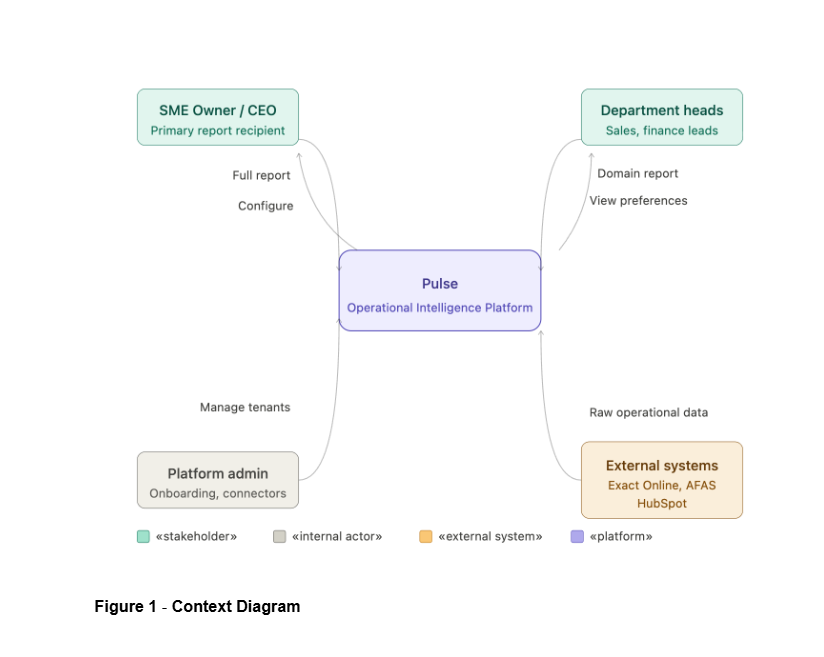
\includegraphics[keepaspectratio]{images/Context_diagram.png}}

}

\caption{\label{fig-context-diagram}Context Diagram}

\end{figure}%

\begin{figure}

\centering{

\pandocbounded{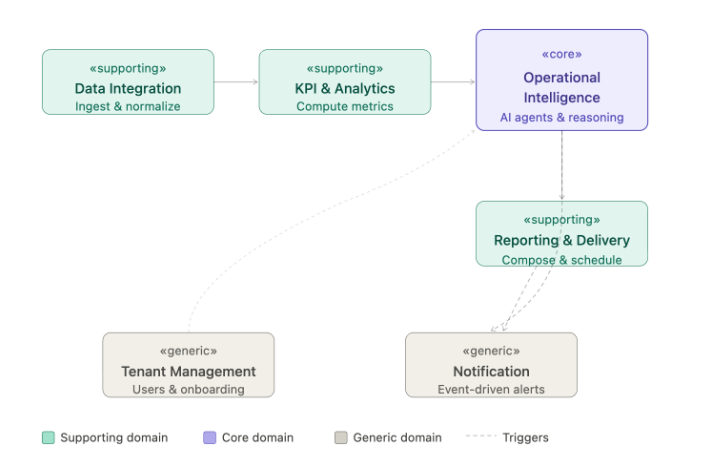
\includegraphics[keepaspectratio]{images/Figure 2 Domain Diagram.png}}

}

\caption{\label{fig-domain-diagram}Domain Diagram}

\end{figure}%

\begin{figure}

\centering{

\pandocbounded{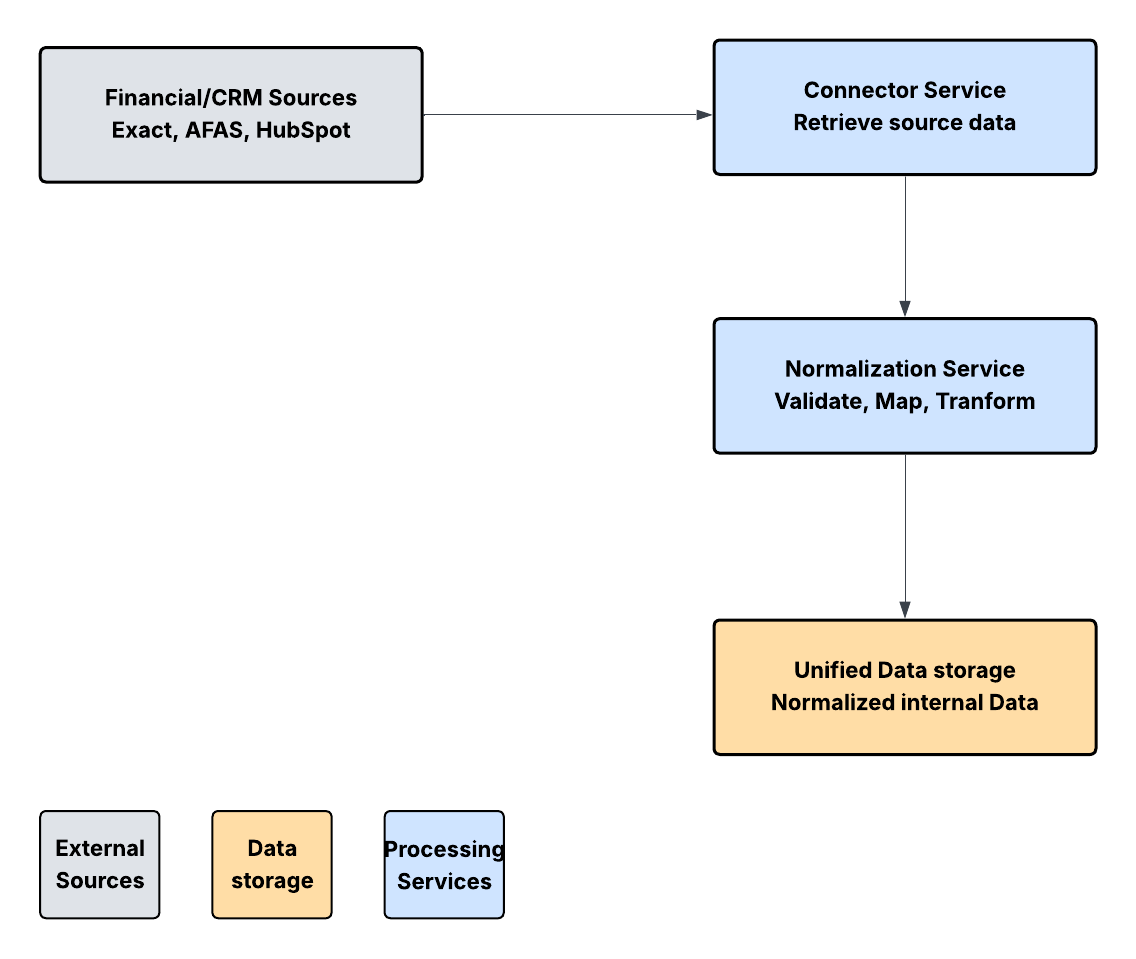
\includegraphics[keepaspectratio]{images/Context Diagram Data integration service.png}}

}

\caption{\label{fig-data-integration}Data Integration Service}

\end{figure}%




\end{document}
